\documentclass[border=3pt,tikz]{standalone}
\usepackage{amsmath} % for \dfrac
\usepackage{physics,siunitx}
\usepackage{tikz,pgfplots}
\usetikzlibrary{angles,quotes} % for pic (angle labels)
\usetikzlibrary{decorations.markings}
\tikzset{>=latex} % for LaTeX arrow head
\usepackage{xcolor}
\colorlet{Rcol}{green!60!black}
\colorlet{myblue}{blue!70!black}
\colorlet{myred}{red!70!black}
\colorlet{Ecol}{orange!90!black}
\tikzstyle{Rline}=[Rcol,thick]
\tikzstyle{gline}=[Rcol,thick]
\tikzstyle{bline}=[myblue,thick]
\tikzstyle{rline}=[myred,thick]
\def\xmax{4.5}
\def\ymax{3}
\def\tick#1#2{\draw[thick] (#1) ++ (#2:0.03*\ymax) --++ (#2-180:0.06*\ymax)}
\newcommand\EMF{\mathcal{E}} %\varepsilon}

\begin{document}
    % Circuito RC: Descarga de Q
    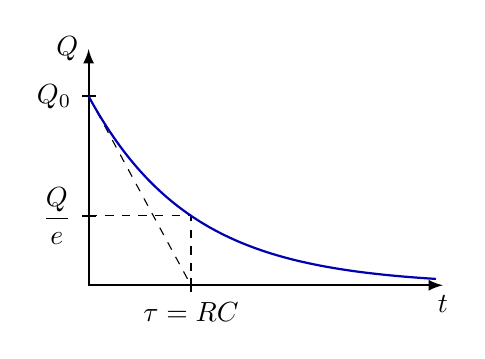
\begin{tikzpicture}
      \def\a{2.4}
      \def\t{1.3}
      \coordinate (O) at (0,0);
      \coordinate (X) at (\xmax,0);
      \coordinate (Y) at (0,\ymax);
      \coordinate (Q) at (0,\a);
      \coordinate (T) at (\t,\a/2.718);
      \coordinate (Tx) at (\t,0);
      \coordinate (Ty) at (0,\a/2.718);
      
      % AXIS
      \draw[<->,thick]
        (X) node[below] {$t$} -- (O) -- (Y) node[left] {$Q$};
      \tick{Q}{0} node[left] {$Q_0$};
      \tick{Tx}{90} node[below] {$\tau = RC$};
      \tick{Ty}{0} node[left] {$\dfrac{Q}{e}$};
      
      % PLOT
      \draw[dashed] (Q) -- (Tx);
      \draw[dashed] (Ty) -- (T) -- (Tx);
      \draw[bline,samples=100,smooth,variable=\x,domain=0:0.98*\xmax]
        plot(\x,{\a*exp(-\x/\t)});
      
    \end{tikzpicture}
    
    
    % Circuito RC: Carga de Q
    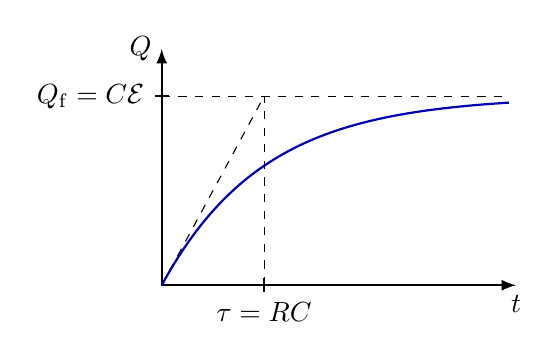
\begin{tikzpicture}
      \def\a{2.4}
      \def\t{1.3}
      \coordinate (O) at (0,0);
      \coordinate (X) at (\xmax,0);
      \coordinate (Y) at (0,\ymax);
      \coordinate (Q) at (0,\a);
      \coordinate (T) at (\t,\a);
      \coordinate (Tx) at (\t,0);
      
      % AXIS
      \draw[<->,thick]
        (X) node[below] {$t$} -- (O) -- (Y) node[left] {$Q$};
      \tick{Q}{0} node[left] {$Q_\mathrm{f} = C\EMF$};
      \tick{Tx}{90} node[below] {$\tau = RC$};
      
      % PLOT
      \draw[dashed] (Q) --++ (0.98*\xmax,0);
      \draw[dashed] (Tx) -- (T);
      \draw[dashed] (O) -- (T);
      \draw[bline,samples=100,smooth,variable=\x,domain=0:0.98*\xmax]
        plot(\x,{\a*(1-exp(-\x/\t)});
      
    \end{tikzpicture}


\end{document}